\section{Methods}\label{s:design}

The study utilizes a digital experiment built with OpenSesame \footnote{code and data available at \url{https://github.com/michelexyz/salient_colors}}. Participants accessed our experiment on the jatos online platform. \footnote{\url{https://jatos.mindprobe.eu/publix/vPrNUgNpaTd}.} Participants sit in front of a computer or laptop and are shown images of a digital football match for 750 milliseconds, followed by a prompt asking them to identify the team they believe had a greater number of players. We chose 750 milliseconds as the time interval because we found empirically that this value would give us an accuracy of about 75\%, as confirmed by the data, for which we could see the maximum degree of effect if present.

\subsection{The Participants}
The experiment was conducted on 49 participants, aged 19 to 61 years, with one outlier at 169, which may be an erroneous entry. There were 33 male participants, 15 females, and 1 other. Majority of the participants do not have impaired vision - only a few reported having impaired vision with a value of "yes." The most common experiences with football are "last-month", and "more". The favorite team responses are varied, with the most being "other" and "blue" being slightly higher than red. "Other" is also the most common favorite color, and "blue" also had more responses than "red".

\subsection{The Intake Form}

In the beginning of the experiment, there is an intake form in the first screen that asks for a user's name, age, gender, if they have a vision is impaired such that their perception of blue or red is affected, when  have they last watched or played football. At the end of the experiment, there are two follow up questions - whether blue the participant's favorite color and the jersey color of their favorite football team. 

These are suspected to be confounding factors and are recorded to be incorporated into the data analysis to allow us to isolate insights while accounting for potential external influences.


\subsection{The Stimuli Used}
In this experiment, we utilized screenshots from the video game "EAFC 24" (formerly known as FIFA) as stimuli.
What made these images unique is that both teams were wearing light blue uniforms (Italy-international kit). We started with 30 images with all the team players in light blue uniforms and used Photoshop to create 60 images from them - 30 with more red players and 30 with more blue players. These new images showed the same game situations and formations but with the teams wearing opposite colors. Thus, if the first image had 7 blue players and 6 red players in one spot, the new image would have 7 red players and 6 blue players (in the same place and in the same location but with swapped shirts). This was helpful because it is very hard and nearly impossible to get the original 30 images duplicated at the same position and scenario in EAFC as there is no option to swap shirts mid game, and we wanted to eliminate any confounding factors in various groupings that may arise from randomly generating all 60 stimuli with the two team colors.

These screenshots depict a match where teams don red and blue uniforms. Our primary objective is to use these images to evaluate participants' perceptions and judgments throughout the study. An illustrative screenshot is available in Figure \ref{fitness1}. There are 30 scenes in total, of which 7 scenes contain 11 players, 4 contain 12 players, 18 contain 13 players and 1 contains 14 players. For 25 scenes, the team sizes differed by 1 players, for 5 scenes it differed by 2. 
To minimize confounding factors, for each scenes, two versions are created - majority red and majority blue. This ensures each scene is presented in identical setups (groupings, poses, etc) but only the color is swapped. The HSL, which is Hue Saturation Value (Brightness) for a sample of blue from the player's shirt is 220deg 100\% 77\%. The HSL for red players is 2deg 100\% 75\%. The HSL value for the green of the field is 94deg 60\% 55\%. This means that the difference of the players jerseys from the color of the field is generally the same. The HSL model, unlike the RGB model, is particularly oriented toward human perspective. 

\begin{figure}[h!]
    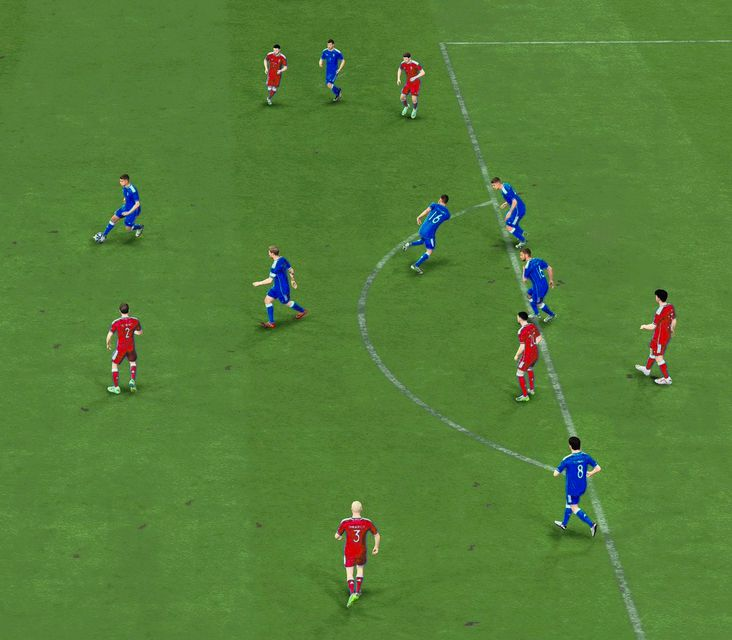
\includegraphics[width=.48\columnwidth]{vu-is-research-thesis/resources/id10_v2_b7_r6.jpg}
    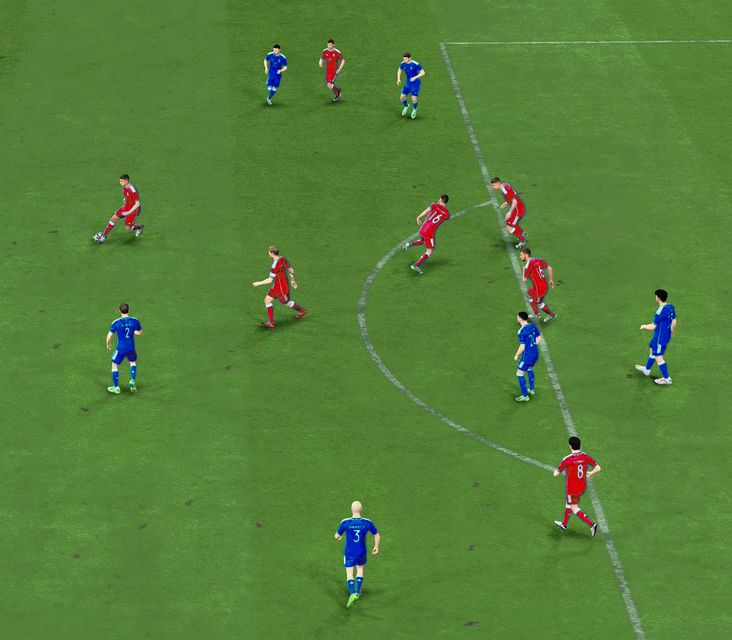
\includegraphics[width=.48\columnwidth]{vu-is-research-thesis/resources/id10_v1_b6_r7.jpg}
    \centering 
   \caption{one scene results in two stimuli where the team colours are swapped}
   \label{fitness1}
\end{figure}

\subsection{The Participant's Task}

After filling out the intake form to gather participants' relevant background information, participants are shown 60 "EAFC 24" screenshots of football players. The participants' primary task in this experiment is to make a judgment regarding which team they believe has a greater number of players in the screenshot they are shown. This task aims to gauge participants' ability to identify the majority team and quantify to what extent is the accuracy depends on jersey colour of the majority team. The mechanics of the experiment are streamlined for precision. Each screenshot is displayed for a brisk 750 milliseconds, a span allowing for instinctual, snap judgments without sufficient time to consciously count the players. Following this brief exposure, participants are prompted to indicate their choice, red or blue. Every response and response time are logged for analysis.